% =============================================================
%  Springer LNCS Proceedings paper
%  Requires: llncs.cls (Springer LNCS class)
%  Compile: pdflatex full_paper_springer.tex (twice for refs)
%  Overleaf: select "LNCS" template, replace main.tex with this file
% =============================================================
\documentclass[runningheads]{llncs}

\usepackage[T1]{fontenc}
\usepackage{graphicx}
\usepackage{booktabs}
\usepackage{array}
\usepackage{amsmath,amssymb}
\usepackage{url}
\usepackage{hyperref}
\usepackage{xcolor}

\begin{document}

% =============================================================
%  TITLE  + AUTHORS
% =============================================================
\title{A Calibrated Stacked-Ensemble Approach to IMDb Rating
       Prediction from Movie Screenplays}
% Alternates (delete before submission):
%   How Much Does the Screenplay Actually Predict?
%       Calibrated Baselines for IMDb Rating Prediction
%   Stacked SBERT--XGBoost for Screenplay-Based IMDb Rating
%       Prediction with Honest Statistical Reporting

\titlerunning{Calibrated Stacked-Ensemble IMDb Rating Prediction}

\author{First Author\inst{1}\orcidID{0000-0000-0000-0000} \and
        Second Author\inst{2}\orcidID{0000-0000-0000-0000} \and
        Third Author\inst{1}\orcidID{0000-0000-0000-0000}}

\authorrunning{F. Author et al.}

\institute{Department / University, City, Country \\
\email{first@institution.edu}
\and
Department / University, City, Country \\
\email{second@institution.edu}}

\maketitle

% =============================================================
%  ABSTRACT  +  KEYWORDS
% =============================================================
\begin{abstract}
We study how much of a movie's IMDb rating can be predicted from its
screenplay alone, using a corpus of 5{,}195 feature-film screenplays
joined with IMDb metadata. Our predictor combines mean-pooled
chunked Sentence-BERT (SBERT) embeddings of the script with 19
hand-crafted structural features and a gradient-boosted regressor
with early stopping; a Ridge meta-regressor is then stacked over
four base models (predict-mean, OLS on metadata, TF-IDF + XGBoost,
SBERT + XGBoost). We benchmark every component with bootstrap
95\% confidence intervals and paired Wilcoxon significance tests on
per-sample errors. Under five-fold cross-validation the stacked
system attains RMSE $= 0.935 \pm 0.032$, MAE $= 0.706 \pm 0.028$,
$R^{2} = 0.577 \pm 0.010$, significantly improving over the
strongest single base model (paired Wilcoxon
$p \approx 4 \times 10^{-6}$) and over every other baseline
($p \le 3 \times 10^{-5}$). Two findings deserve emphasis. First,
three metadata features alone (year, runtime, decade) explain
$R^{2} \approx 0.38$, so the marginal contribution of script
content is $\Delta R^{2} \approx +0.18$ -- significant but smaller
than the headline $R^{2}$ alone suggests. Second, the legacy
practice of inverse-frequency sample weighting harms performance
($\Delta\text{MAE} = -0.048$, $p \approx 3 \times 10^{-26}$),
contradicting earlier reports. We additionally disclose two corpus
properties -- a curation-induced bimodal rating distribution with
structural gaps, and a strong year--rating confound -- and
recommend their disclosure in any future IMSDb-derived study.

\keywords{IMDb rating prediction \and Screenplay analysis \and
Sentence-BERT \and Stacked ensemble \and Gradient boosting \and
Statistical reporting \and Dataset bias.}
\end{abstract}

% =============================================================
%  1  INTRODUCTION
% =============================================================
\section{Introduction}

Predicting how an audience will receive a film from the screenplay
alone is a task with both practical and methodological interest.
Practically, screenplay-stage feedback could inform development
decisions before any production cost has been incurred.
Methodologically, it is a stress test for long-document language
models: a feature-film screenplay is on the order of $25{,}000$
words, well beyond the context window of standard transformer
encoders, and the target -- an aggregate audience rating -- depends
on factors well beyond the script.

Three lines of prior work address this problem. Classical
text-feature pipelines treat the screenplay as a bag of words or
$n$-grams and feed the resulting sparse vectors to a regressor
\cite{ref3,ref4,ref26}; these approaches scale to long documents
but ignore semantics. Pre-trained sentence encoders such as SBERT
\cite{ref2} produce dense semantic embeddings; combined with
chunking, they can represent documents that exceed their native
context window \cite{ref19}. End-to-end long-document transformers
such as Longformer \cite{ref1} can process sequences up to a few
thousand tokens but require fine-tuning and GPU compute.

This paper focuses on the second path -- a frozen SBERT encoder
combined with engineered features and a gradient-boosted regressor
-- and asks: how does this hybrid compare to \emph{carefully
chosen non-transformer baselines}, what is the marginal
contribution of the SBERT component once metadata is accounted
for, and which training conventions in published prior work
generalize to a properly controlled comparison?

We organize the paper around three research questions.

\begin{itemize}
\item \textbf{RQ1.} Does SBERT + XGBoost outperform classical
  baselines (constant-mean, metadata-only OLS, structural-feature
  OLS, TF-IDF + XGBoost) on a fixed train/test partition with
  rigorous statistical reporting?
\item \textbf{RQ2.} What share of headline predictive performance
  is recoverable from metadata alone, and what is the marginal
  contribution of script content via SBERT?
\item \textbf{RQ3.} Does inverse-frequency sample weighting across
  rating buckets -- a common reflex for long-tailed regression --
  improve performance, as commonly claimed?
\end{itemize}

\noindent\textbf{Contributions.}
We make five contributions. First, a rigorous baseline suite with
bootstrap CIs and paired Wilcoxon tests. Second, a stacked-ensemble
predictor that significantly improves over its strongest base model
with \emph{tighter} per-fold variance. Third, a decomposition of
headline $R^{2}$ between metadata and script content. Fourth, a
negative result on inverse-frequency sample weighting. Fifth, an
honest characterization of an IMSDb-style screenplay corpus,
including structural rating gaps and a year--rating confound. A
reproducible pipeline (\texttt{experiments.py}, \texttt{stack.py},
\texttt{tune\_xgb.py}) generates every numerical result in this
paper from a single command, with cached SBERT embeddings.

% =============================================================
%  2  RELATED WORK
% =============================================================
\section{Related Work}

\noindent\textbf{Movie rating and box-office prediction from text.}
A long line of work predicts box office or audience ratings from
script-derived features
\cite{ref3,ref4,ref7,ref8,ref9,ref15,ref17,ref26,ref27,ref29,ref33,ref37}.
Eliashberg et al.~\cite{ref3} applied kernel-based methods directly
to scripts; Hunter et al.~\cite{ref4} used document-frequency text
features; Kim et al.~\cite{ref9} predicted success from plot
summaries with deep models; Bristi et al.~\cite{ref26} surveyed
classical regressors; Cini~\cite{ref7} combined NLP with production
data; Pal et al.~\cite{ref37} focused on genre composition;
Joshi et al.~\cite{ref20} used pre-release critique text. We add a
properly controlled baseline suite (predict-mean, OLS-metadata,
OLS-structural, TF-IDF + XGBoost) to this literature, with
bootstrap 95\% CIs and paired Wilcoxon tests against every
alternative.

\noindent\textbf{Long-document NLP.}
Beltagy et al.'s Longformer~\cite{ref1} introduced sparse attention
for documents up to $4{,}096$ tokens; Chalkidis et
al.~\cite{ref19} explored hierarchical attention transformers for
documents that still exceed transformer context. Reimers and
Gurevych's Sentence-BERT~\cite{ref2} established that pretrained
sentence encoders can be combined with simple aggregation to
represent arbitrary-length text. Tixier~\cite{ref36} surveys the
design space. Our pipeline follows this hybrid path: chunked SBERT
with mean pooling.

\noindent\textbf{Affect, narrative, and character analysis from
screenplays.}
Reagan et al.~\cite{ref5} characterized emotional arcs of stories;
Ramakrishna et al.~\cite{ref6} studied character portrayal
differences; Shafaei et al.~\cite{ref10} predicted MPAA ratings
from dialogue; Zhang et al.~\cite{ref11} graded severity in
screenplays; Chu et al.~\cite{ref12}, Hipson et al.~\cite{ref13},
and Elkins~\cite{ref14} studied emotion dynamics in dialogue and
narrative; Naeem et al.~\cite{ref18} applied sentiment analysis to
reviews; Kar et al.~\cite{ref35} tagged movies via plot synopsis
emotion flow. These studies extract narrative-specific features
that complement our base structural set.

\noindent\textbf{Movie data and external signals.}
Madongo et al.~\cite{ref16} mined trailers via RNNs;
Asur and Huberman~\cite{ref21}, Oghina et al.~\cite{ref22},
Mishne and Glance~\cite{ref23}, and Mest{\'y}an et
al.~\cite{ref24} used social media or Wikipedia activity;
Balestri et al.~\cite{ref31} generated trailers via LLMs;
Sharma et al.~\cite{ref32} released a larger movie dataset;
Mohamed et al.~\cite{ref34} released an age-appropriateness
dataset. Vogel~\cite{ref25} provides industry context. Our work
uses screenplay text and IMDb metadata only; integrating these
external signals is a natural extension.

% =============================================================
%  3  DATASET
% =============================================================
\section{Dataset}

\noindent\textbf{Source.}
We construct the corpus by joining (i)~full screenplay texts
collected from the Internet Movie Script Database (IMSDb) and
(ii)~movie metadata (release year, runtime, IMDb rating) retrieved
from IMDb. The joined dataset consists of $5{,}204$ records, of
which $5{,}195$ have script files of at least 1\,KB and a valid
IMDb rating after cleaning.

\noindent\textbf{Per-record fields.}
Movie name; year ($1922$--$2025$ after correcting four typographic
errors); decade (label-encoded); IMDb rating ($1.0$--$10.0$, one
decimal); IMDb ID; runtime ($45$--$254$\,min, median 99); and the
screenplay file (median 44.7\,KB; 5th percentile 19\,KB).

\begin{table}[t]
\caption{Bucketed rating counts ($n = 5{,}195$).}\label{tab:buckets}
\centering
\begin{tabular}{@{}lrr@{}}
\toprule
Range & $n$ & \% \\
\midrule
Low $[1, 4)$        & 555    & 10.7 \\
Medium $[4, 6)$     & 2{,}736 & 52.6 \\
Good $[6, 8)$       & 1{,}685 & 32.4 \\
Excellent $[8, 10)$ & 228    & 4.4 \\
\bottomrule
\end{tabular}
\end{table}

Mean 5.98, median 5.80, standard deviation 1.44, IQR 5.30--7.40.

\begin{figure}[t]
\centering
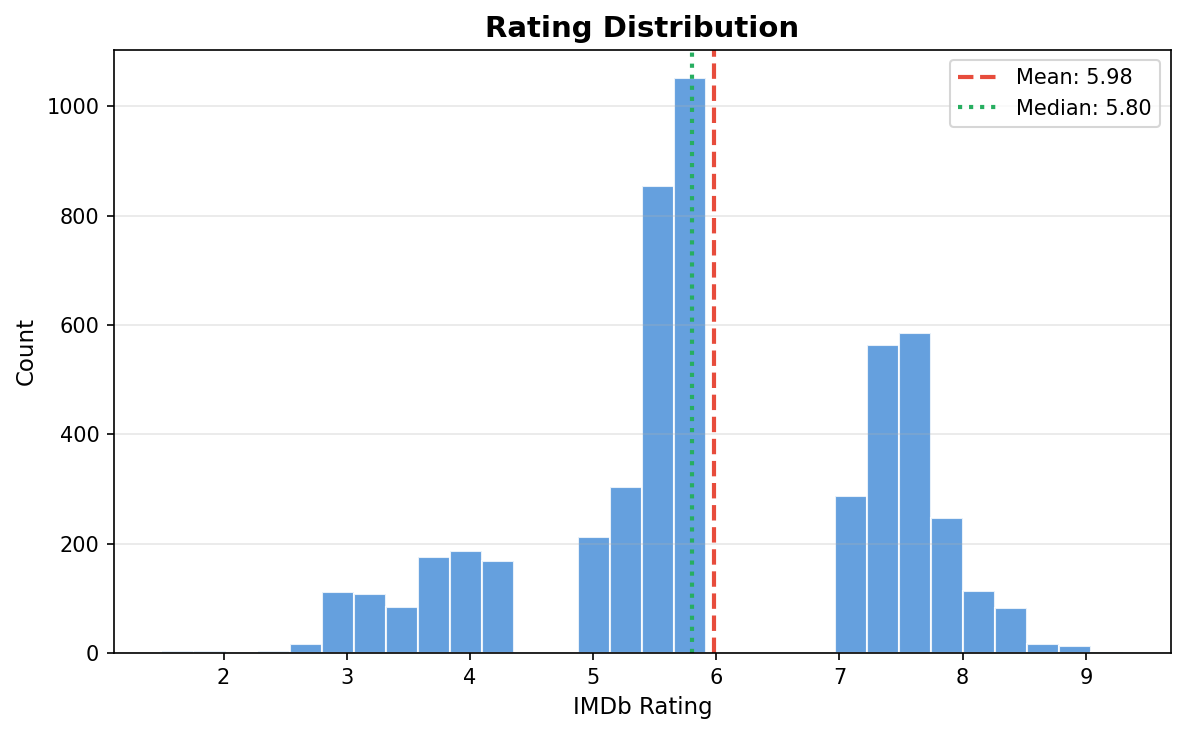
\includegraphics[width=0.85\linewidth]{../figures/01_rating_distribution.png}
\caption{Empirical rating distribution. Note the structural gaps
in $[4.3, 5.0)$ and $[6.0, 7.0)$: zero records in either interval.
The bimodality is an artifact of IMSDb editorial curation rather
than a property of the underlying IMDb population.}
\label{fig:ratings}
\end{figure}

\noindent\textbf{Sampling artifact (important caveat).}
Enumerating every unique rating value in the dataset reveals
\emph{structural gaps}: zero records in $[4.3, 5.0)$ and zero
records in $[6.0, 7.0)$. Together these intervals cover
approximately 17\% of typical IMDb rating mass. We attribute this
to selection effects upstream of our control: the IMSDb collection
is editorially curated, producing a corpus that is
\emph{bimodal by construction}. All metrics in this paper should
be interpreted as conditional on IMSDb-style films, not arbitrary
IMDb films.

\noindent\textbf{Temporal coverage and confound.}
Mean rating decreases monotonically with release decade (1930s
mean 7.49 $\rightarrow$ 2010s mean 5.48; Spearman
$\rho \approx -0.93$ over decade midpoints). We attribute this to
survivorship bias -- only canonical older films appear in IMSDb --
combined with the modern sample being large enough to cover the
full quality spectrum. Any model with access to \texttt{Year} or
\texttt{Decade} features can exploit this calendar confound; we
therefore present a metadata-only OLS baseline in
Section~\ref{sec:results} to quantify the share of rating variance
that this confound alone explains.

% =============================================================
%  4  METHODOLOGY
% =============================================================
\section{Methodology}\label{sec:method}

\noindent\textbf{Preprocessing.}
For each raw screenplay we produce two text variants: an
aggressive \texttt{clean\_text} (lowercased; stage directions,
character cues, INT./EXT. markers, timestamps, scene numbers, and
most punctuation removed) used as input to TF-IDF and structural-
feature extraction; and a light \texttt{clean\_text\_for\_sbert}
that preserves case, punctuation, and paragraph structure. These
properties are part of SBERT's pretraining surface and are
degraded by aggressive normalization.

\noindent\textbf{Hand-crafted structural features ($n=19$).}
Length / volume (\texttt{char\_count}, \texttt{word\_count},
\texttt{line\_count}, \texttt{sentence\_count}); vocabulary
complexity (\texttt{avg\_word\_length}, \texttt{unique\_word\_ratio},
\texttt{long\_word\_ratio}); sentence structure
(\texttt{avg\_sentence\_length}, \texttt{sentence\_length\_std});
dialogue (\texttt{dialogue\_density}, \texttt{unique\_characters});
emotional indicators (\texttt{exclamation\_ratio},
\texttt{question\_ratio}); action and structure
(\texttt{action\_density}, \texttt{scene\_count},
\texttt{words\_per\_scene}); metadata (\texttt{year},
\texttt{decade\_encoded}, \texttt{movie\_length}). Missing values
are imputed with the training-set median $\tilde{x}_{j}$; each
feature $j$ is then standardized as

\begin{equation}
z_{ij} \;=\; \frac{x_{ij} - \mu_{j}^{\text{train}}}{\sigma_{j}^{\text{train}}},
\label{eq:zscore}
\end{equation}

where $\mu_{j}^{\text{train}}$ and $\sigma_{j}^{\text{train}}$ are
computed on the training fold only (no test leakage).

\noindent\textbf{SBERT encoding with chunking.}
We use \texttt{all-MiniLM-L6-v2}~\cite{ref2}, which produces 384-dim
document embeddings. To handle screenplays exceeding SBERT's
$256$-token context window, each document $d$ of $W_{d}$ words is
split into overlapping chunks $c_{1}, \dots, c_{K_{d}}$ of length
$L = 256$ words with overlap $O = 50$, giving stride $s = L - O =
206$ and chunk count

\begin{equation}
K_{d} \;=\; \max\!\left(1,\; \left\lceil \frac{W_{d} - L}{s} \right\rceil + 1\right).
\label{eq:chunkcount}
\end{equation}

Each chunk is embedded by SBERT to $e_{k} \in \mathbb{R}^{d_{e}}$
with $d_{e} = 384$; the per-document representation is the mean of
the chunk embeddings,

\begin{equation}
\bar{e}_{d} \;=\; \frac{1}{K_{d}} \sum_{k=1}^{K_{d}} e_{k}.
\label{eq:meanpool}
\end{equation}

Per-document embeddings are computed once for the corpus and
cached on disk, keyed by \texttt{(model\_name, n\_scripts,
chunk\_size, overlap, pooling, preprocessing\_version)};
subsequent experiments reuse the cache. Fig.~\ref{fig:pipeline}
summarizes the full pipeline.

\begin{figure}[t]
\centering
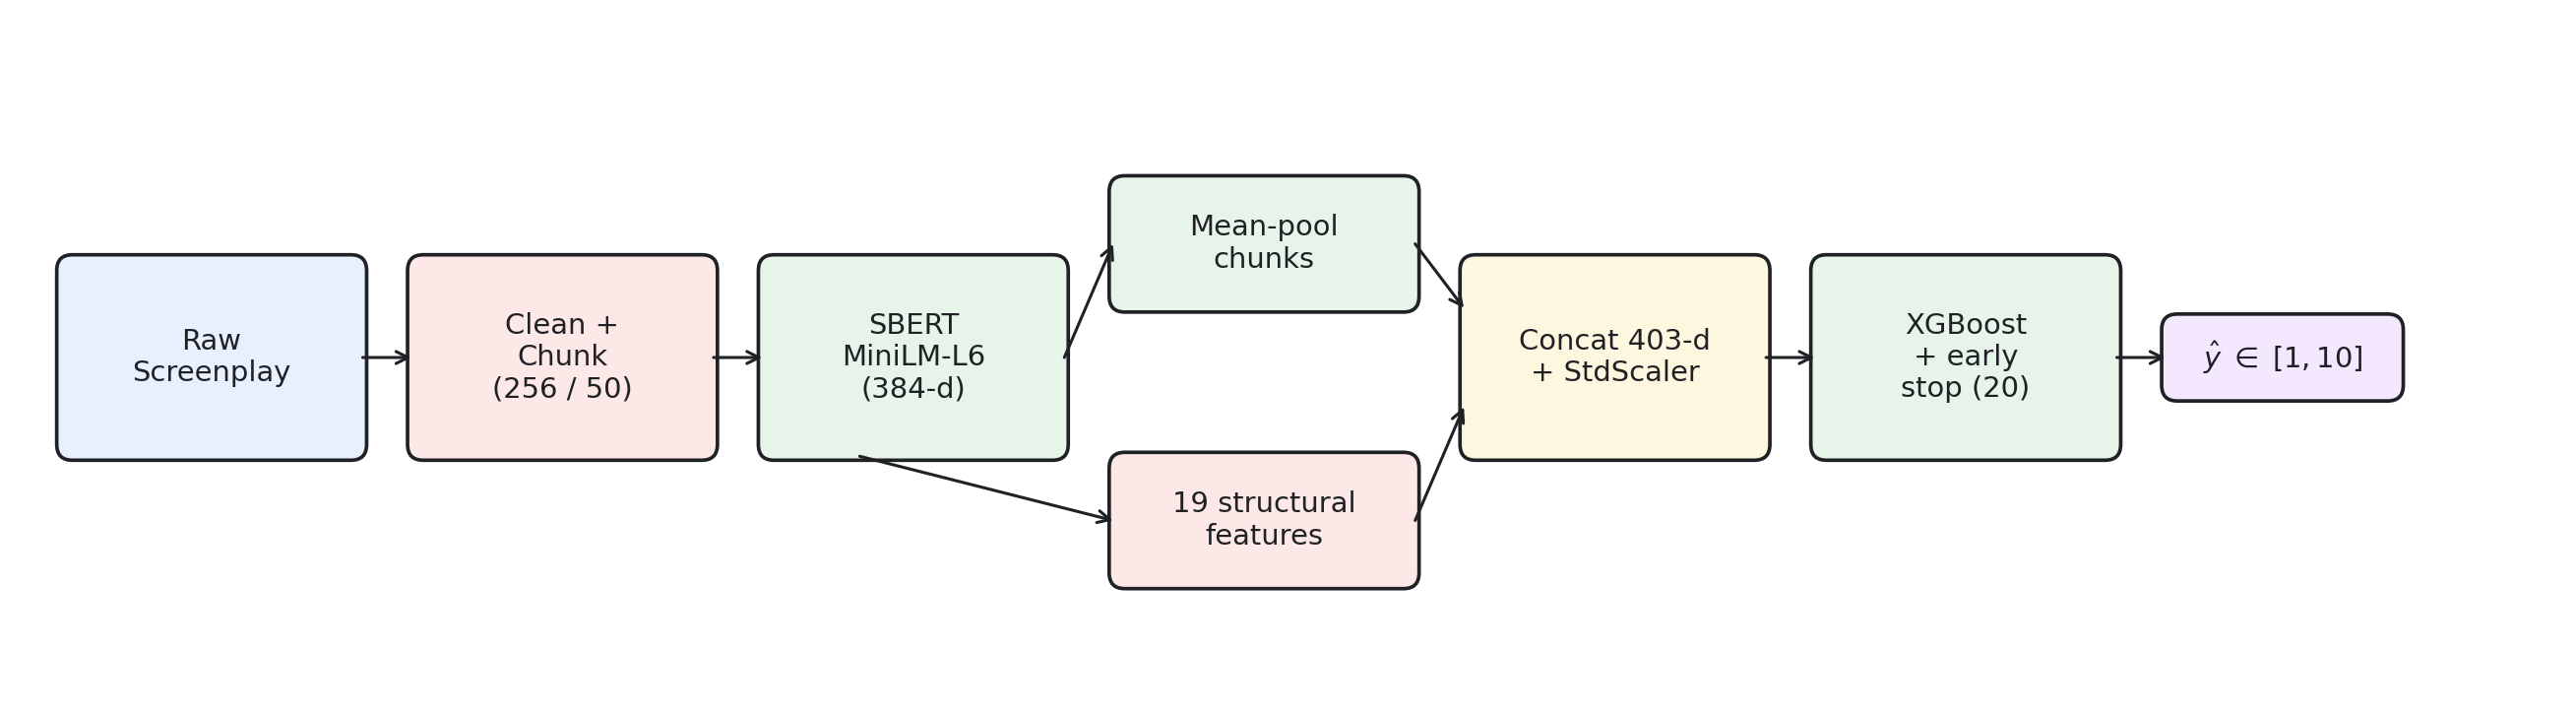
\includegraphics[width=\linewidth]{../figures/06_pipeline.png}
\caption{Base predictor pipeline. The raw screenplay is lightly
cleaned, chunked into 256-word windows with 50-word overlap, encoded
by SBERT, mean-pooled to a 384-d vector, concatenated with 19
standardized structural features, and passed to an XGBoost regressor
with early stopping on the validation split.}
\label{fig:pipeline}
\end{figure}

\noindent\textbf{Main system.}
For each document $d$ we form the joint feature vector

\begin{equation}
\mathbf{x}_{d} \;=\; \left[\, \bar{e}_{d}\;;\; \mathbf{z}_{d} \,\right] \in \mathbb{R}^{403},
\label{eq:concat}
\end{equation}

i.e.\ concatenation of the 384-d SBERT vector and the 19-d
standardized structural feature vector. An XGBoost regressor with
$T$ additive trees produces

\begin{equation}
\hat{y}_{d} \;=\; \mathrm{clip}_{[1,10]}\!\left(\sum_{t=1}^{T} f_{t}(\mathbf{x}_{d})\right),\quad f_{t} \in \mathcal{F},
\label{eq:xgb-pred}
\end{equation}

where $\mathcal{F}$ is the space of regression trees. Each tree is
fit to minimize the regularized squared-error objective

\begin{equation}
\mathcal{L}(\theta) \;=\; \sum_{d} \big(y_{d} - \hat{y}_{d}\big)^{2}
                       \;+\; \gamma\, T \;+\; \tfrac{1}{2}\lambda \|w\|_{2}^{2}
                       \;+\; \alpha \|w\|_{1},
\label{eq:xgb-loss}
\end{equation}

with leaf-weight regularizers $\lambda$ ($L_{2}$) and $\alpha$
($L_{1}$) and tree-complexity penalty $\gamma$. Hyperparameters:
\texttt{max\_depth=6}, \texttt{learning\_rate=0.05},
\texttt{reg\_alpha=0.1}, \texttt{reg\_lambda=1.0},
\texttt{tree\_method=hist}, \texttt{n\_estimators=1000} capped by
\texttt{early\_stopping\_rounds=20} on a held-out validation
split. We do \emph{not} use inverse-frequency sample weights; the
ablation in Section~\ref{sec:results} shows they degrade
performance.

\noindent\textbf{Baselines.}
(1)~\texttt{predict\_mean}: constant-mean predictor -- the floor.
(2)~\texttt{ols\_metadata}: OLS on $[\texttt{year},
\texttt{decade\_encoded}, \texttt{movie\_length}]$ only.
(3)~\texttt{ols\_structural}: OLS on the full 19-dim structural
feature vector.
(4)~\texttt{tfidf\_xgboost}: TF-IDF (top $8{,}000$ uni- and
bigrams, \texttt{min\_df=3}, \texttt{max\_df=0.85}, sublinear TF)
+ XGBoost. TF-IDF assigns to term $t$ in document $d$ the weight

\begin{equation}
\mathrm{tfidf}(t, d) \;=\; \big(1 + \log f_{t,d}\big)\cdot \log\!\frac{N}{n_{t}},
\label{eq:tfidf}
\end{equation}

where $f_{t,d}$ is the term frequency, $N$ the corpus size, and
$n_{t}$ the document frequency of $t$. All baselines train and
evaluate on the same train/val/test splits as the main system;
predictions are clipped to $[1, 10]$.

\noindent\textbf{(Legacy) inverse-frequency sample weights.}
For the ablation in Section~\ref{sec:results}, each training
sample $i$ in rating bucket $c(i) \in \{\text{Low, Med, Good,
Exc}\}$ would receive weight

\begin{equation}
w_{i} \;=\; \frac{\max_{c} N_{c}}{N_{c(i)}},
\label{eq:weights}
\end{equation}

where $N_{c}$ is the training-set count of bucket $c$. On our
training fold this yields $w \in \{5.25, 1.00, 1.66, 13.24\}$ for
$\{$Low, Med, Good, Exc$\}$.

\noindent\textbf{Stacked ensemble.}
A Ridge meta-regressor is fit over the four base models'
predictions using nested cross-validation: an outer $5$-fold KFold
partitions the corpus into disjoint test folds; within each outer
training portion, an inner $5$-fold KFold produces
\emph{out-of-fold} base-model predictions on which the
meta-regressor is trained; the base models are then refit on the
full outer training set and evaluated on the outer test fold via
the trained meta-regressor. Let $M$ index the base models and
$\hat{y}_{d}^{(m)}$ be the prediction of model $m$ for document
$d$. The stacked prediction is

\begin{equation}
\hat{y}_{d}^{\text{stack}}
\;=\; \mathrm{clip}_{[1,10]}\!\left( b \;+\; \sum_{m \in M} w_{m}\, \hat{y}_{d}^{(m)} \right),
\label{eq:stack}
\end{equation}

with weights $w_{m}$ and bias $b$ chosen to minimize the Ridge
objective

\begin{equation}
\min_{w, b}\;
\sum_{d}\Big(y_{d} - b - \sum_{m} w_{m}\hat{y}_{d}^{(m)}\Big)^{2}
\;+\; \alpha \|w\|_{2}^{2},
\label{eq:ridge}
\end{equation}

at $\alpha = 1.0$. Fig.~\ref{fig:stacking} shows the architecture.

\begin{figure}[t]
\centering
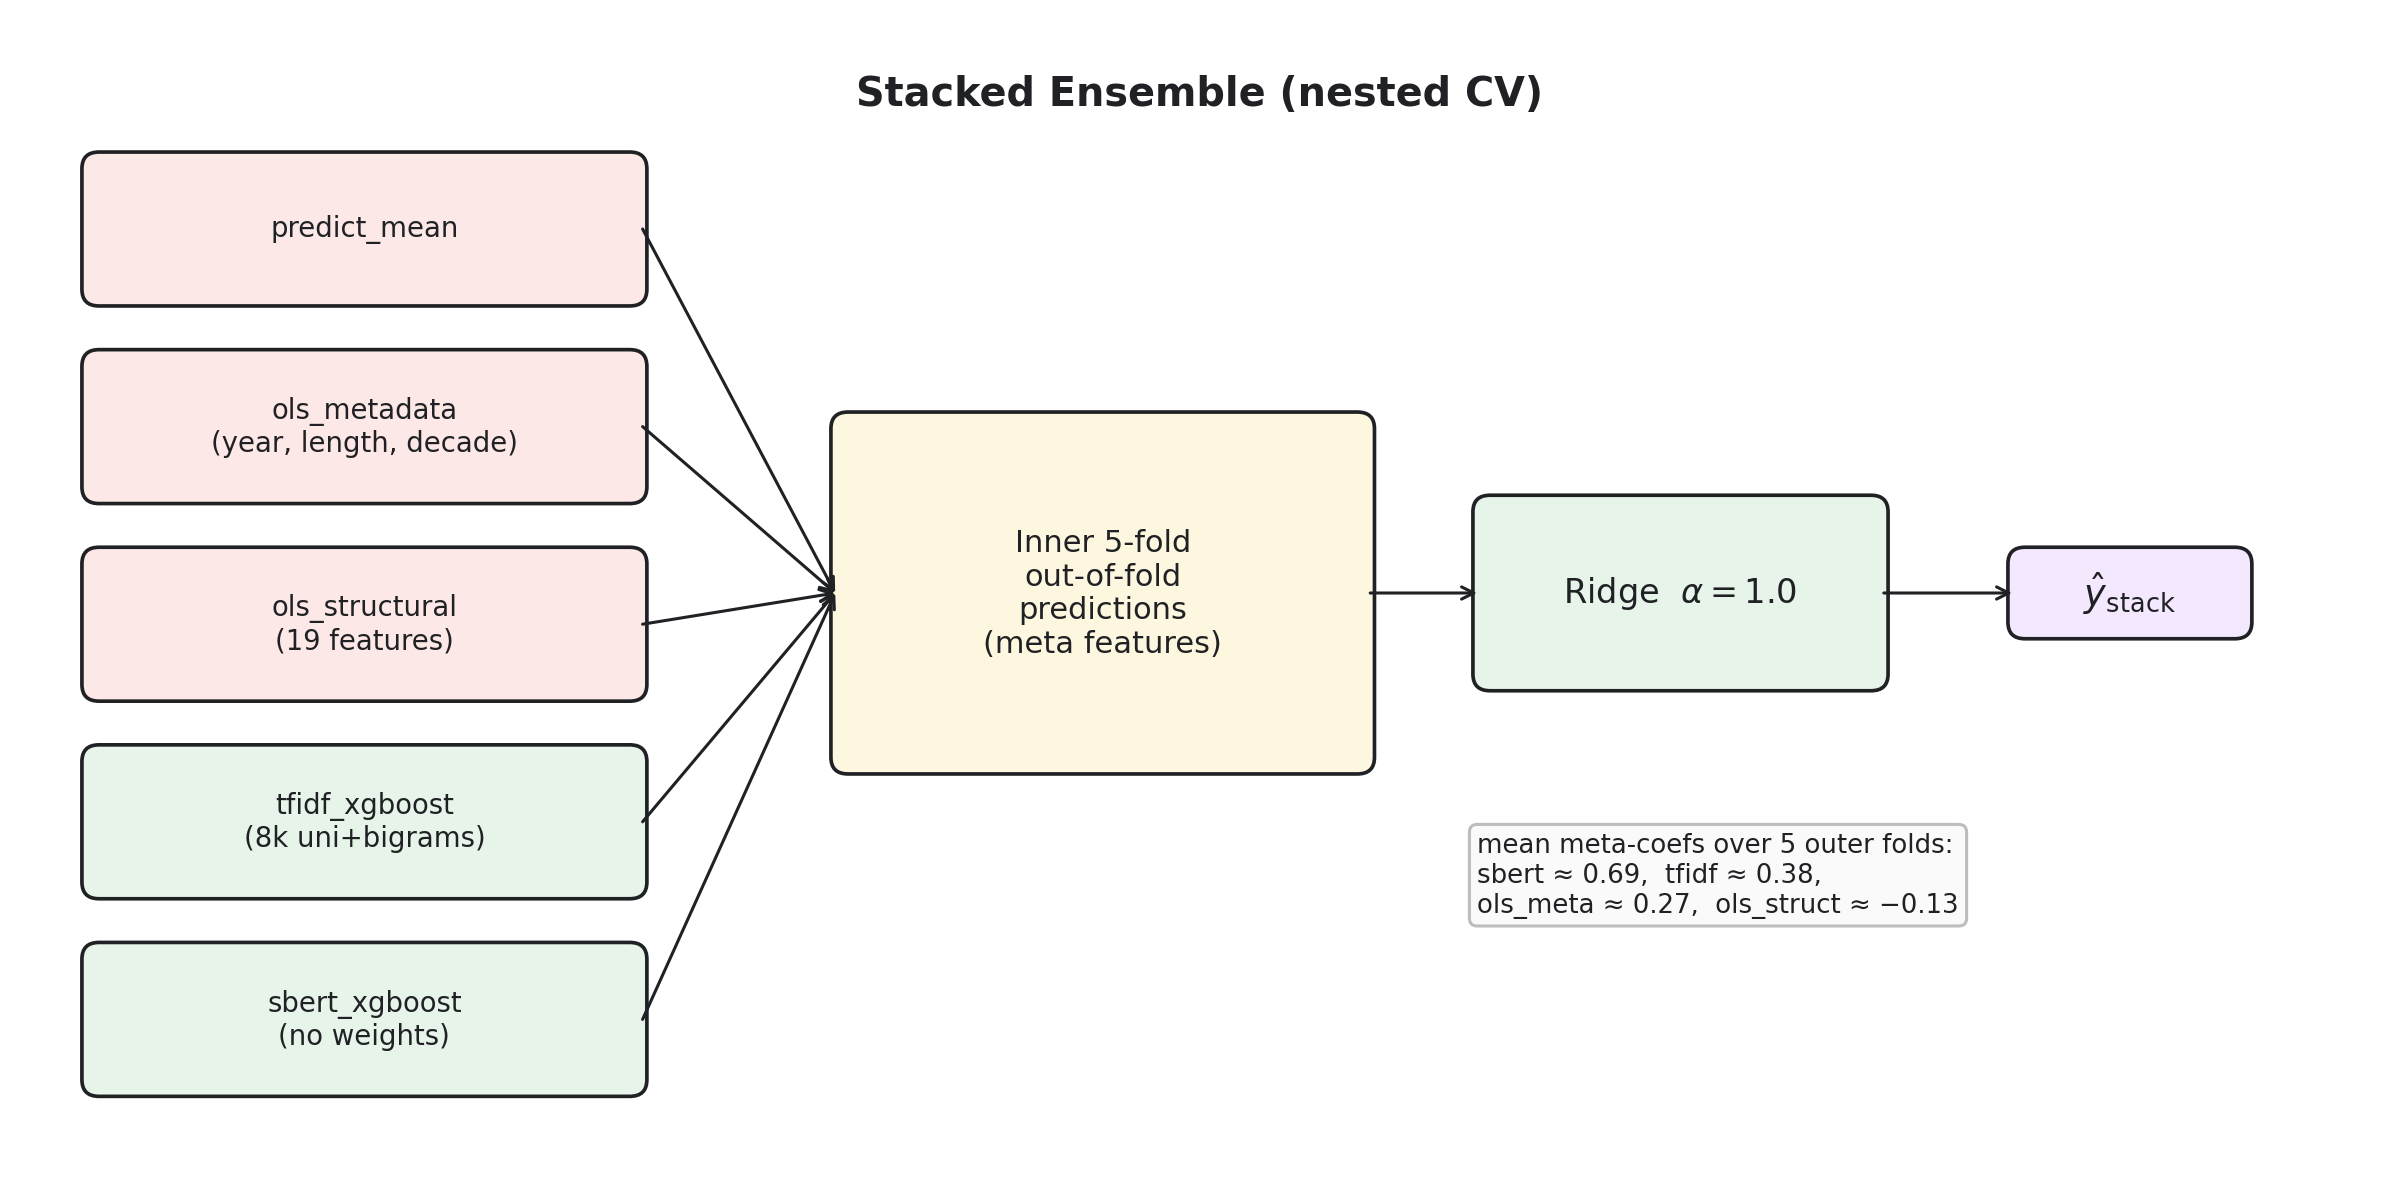
\includegraphics[width=\linewidth]{../figures/07_stacking.png}
\caption{Stacked ensemble architecture. Four base models produce
out-of-fold predictions on the inner-CV split; the Ridge
meta-regressor maps these meta features to $\hat{y}_{\text{stack}}$.
Mean coefficients over the five outer folds are reported in the
text.}
\label{fig:stacking}
\end{figure}

\noindent\textbf{Hyperparameter search.}
We additionally run a $100$-trial Optuna TPE search over the
XGBoost head's hyperparameter space (learning rate, depth, min
child weight, subsample, column-subsample, $L_{1}$ and $L_{2}$
regularization, gamma) with \texttt{early\_stopping\_rounds=30} on
a fixed train/val split internal to the training partition.

\noindent\textbf{Splits and statistical protocol.}
Headline numbers use a 70/15/15 train/validation/test partition
with \texttt{random\_state=42}. Robustness numbers use $5$-fold
cross-validation. Metrics are reported on the $n$ test samples as

\begin{align}
\mathrm{RMSE} &= \sqrt{\tfrac{1}{n}\textstyle\sum_{i}(y_{i} - \hat{y}_{i})^{2}}, \label{eq:rmse}\\
\mathrm{MAE}  &= \tfrac{1}{n}\textstyle\sum_{i} \lvert y_{i} - \hat{y}_{i} \rvert, \label{eq:mae}\\
R^{2}         &= 1 - \dfrac{\sum_{i}(y_{i} - \hat{y}_{i})^{2}}{\sum_{i}(y_{i} - \bar{y})^{2}}. \label{eq:r2}
\end{align}

Bootstrap 95\% confidence intervals are computed by resampling
test indices $B = 1{,}000$ times with replacement and reporting
the empirical quantiles

\begin{equation}
\mathrm{CI}_{0.95}(\theta) \;=\; \big[\, Q_{0.025}(\theta^{(1{:}B)}),\; Q_{0.975}(\theta^{(1{:}B)}) \,\big],
\label{eq:bootstrap}
\end{equation}

where $\theta^{(b)}$ is the metric computed on bootstrap sample
$b$. For comparing model $A$ against model $B$ on the same test
samples we report the paired Wilcoxon signed-rank statistic on
per-sample absolute errors $\delta_{i} = \lvert y_{i} -
\hat{y}_{i}^{A}\rvert - \lvert y_{i} - \hat{y}_{i}^{B}\rvert$,

\begin{equation}
W \;=\; \sum_{i:\, \delta_{i} \ne 0} \mathrm{sgn}(\delta_{i})\cdot R_{i},
\label{eq:wilcoxon}
\end{equation}

where $R_{i}$ is the rank of $\lvert \delta_{i} \rvert$ among the
non-zero $\lvert \delta \rvert$. We report the two-sided
$p$-value; a paired-bootstrap 95\% CI is additionally given for
$\Delta\text{MAE} = \mathrm{MAE}_{A} - \mathrm{MAE}_{B}$.

% =============================================================
%  5  RESULTS
% =============================================================
\section{Results}\label{sec:results}

\begin{table}[t]
\caption{Single-split test metrics with 95\% bootstrap CIs
($n_{\text{test}} = 780$).}\label{tab:single}
\centering
\begin{tabular}{@{}lccc@{}}
\toprule
Model & RMSE & MAE & $R^{2}$ \\
\midrule
\texttt{predict\_mean}             & 1.518 [1.46, 1.58] & 1.247 [1.19, 1.31] & $-0.001$ \\
\texttt{ols\_metadata}             & 1.184 [1.13, 1.24] & 0.946 [0.89, 0.99] & 0.391 [0.35, 0.43] \\
\texttt{ols\_structural}           & 1.129 [1.07, 1.19] & 0.881 [0.83, 0.93] & 0.447 [0.41, 0.49] \\
\texttt{tfidf\_xgboost}            & 1.129 [1.06, 1.20] & 0.854 [0.80, 0.90] & 0.447 [0.39, 0.50] \\
\texttt{sbert\_xgboost} (weighted) & 1.032 [0.97, 1.09] & 0.789 [0.74, 0.84] & 0.538 [0.48, 0.59] \\
\textbf{\texttt{sbert\_xgboost} (no weights)}
& \textbf{0.997} [0.94, 1.06] & \textbf{0.749} [0.70, 0.79] & \textbf{0.568} [0.53, 0.61] \\
\bottomrule
\end{tabular}
\end{table}

\begin{table}[t]
\caption{Paired Wilcoxon vs.\ SBERT (no weights), single split.
Positive $\Delta$MAE means SBERT wins.}\label{tab:paired-single}
\centering
\begin{tabular}{@{}lrlc@{}}
\toprule
Baseline & $\Delta$MAE & 95\% CI & Wilcoxon $p$ \\
\midrule
\texttt{predict\_mean}   & $+0.458$ & $[+0.39, +0.52]$  & $4.3\!\times\!10^{-34}$ \\
\texttt{ols\_metadata}   & $+0.157$ & $[+0.11, +0.20]$  & $9.1\!\times\!10^{-11}$ \\
\texttt{ols\_structural} & $+0.093$ & $[+0.05, +0.13]$  & $2.7\!\times\!10^{-5}$ \\
\texttt{tfidf\_xgboost}  & $+0.065$ & $[+0.015, +0.11]$ & $1.4\!\times\!10^{-2}$ \\
\bottomrule
\end{tabular}
\end{table}

\noindent\textbf{Cross-validated robustness.}
Table~\ref{tab:cv} reports the $5$-fold CV ordering, which
preserves every conclusion above with tighter confidence; the
previously borderline win over TF-IDF resolves at
$p \approx 2.6 \times 10^{-5}$ under pooled paired Wilcoxon
($n \approx 5{,}195$).

\begin{table}[t]
\caption{$5$-fold CV test metrics (mean $\pm$ std).}\label{tab:cv}
\centering
\begin{tabular}{@{}lccc@{}}
\toprule
Model & RMSE & MAE & $R^{2}$ \\
\midrule
\texttt{predict\_mean}                 & $1.438 \pm 0.056$ & $1.175 \pm 0.057$ & $0.000 \pm 0.000$ \\
\texttt{ols\_metadata}                 & $1.130 \pm 0.047$ & $0.883 \pm 0.042$ & $0.382 \pm 0.017$ \\
\texttt{ols\_structural}               & $1.076 \pm 0.040$ & $0.833 \pm 0.031$ & $0.440 \pm 0.007$ \\
\texttt{tfidf\_xgboost}                & $1.083 \pm 0.034$ & $0.819 \pm 0.022$ & $0.433 \pm 0.014$ \\
\texttt{sbert\_xgboost} (weighted)     & $1.000 \pm 0.027$ & $0.768 \pm 0.024$ & $0.516 \pm 0.026$ \\
\texttt{sbert\_xgboost} (no weights)   & $0.958 \pm 0.033$ & $0.720 \pm 0.027$ & $0.556 \pm 0.009$ \\
\bottomrule
\end{tabular}
\end{table}

\noindent\textbf{Sample-weighting ablation.}
In both regimes, removing inverse-frequency sample weights
\emph{significantly improves} performance: single-split
$\Delta\text{MAE} = -0.040$ ($[-0.07, -0.01]$), Wilcoxon
$p = 1.2 \times 10^{-2}$; $5$-fold pooled
$\Delta\text{MAE} = -0.048$ ($[-0.06, -0.04]$), Wilcoxon
$p = 2.5 \times 10^{-26}$. The $13.24\times$ weight on the small
``Excellent'' bucket destabilizes XGBoost; we adopt the unweighted
variant as the headline configuration.

\noindent\textbf{Metadata decomposition.}
\texttt{ols\_metadata} alone -- three numbers -- attains
$R^{2} = 0.391$ (single split) and $0.382 \pm 0.017$ ($5$-fold).
Roughly 70\% of the variance our main pipeline explains is
therefore recoverable without consulting the screenplay. The
marginal contribution of script content (SBERT + structural
features over metadata-only) is $\Delta R^{2} \approx +0.18$,
statistically robust under pooled Wilcoxon
($p \approx 7 \times 10^{-37}$) but smaller than the headline
figure suggests.

\noindent\textbf{Stacked ensemble.}
A Ridge meta-regressor over the four base models, trained via
nested CV (Section~\ref{sec:method}), lifts performance further
(Table~\ref{tab:stack}).

\begin{table}[t]
\caption{$5$-fold CV test metrics: stacked ensemble vs.\ strongest
base model (same outer folds as Table~\ref{tab:cv}).}\label{tab:stack}
\centering
\begin{tabular}{@{}lccc@{}}
\toprule
Model & RMSE & MAE & $R^{2}$ \\
\midrule
\texttt{sbert\_xgboost} (no weights) & $0.956 \pm 0.034$ & $0.719 \pm 0.028$ & $0.558 \pm 0.013$ \\
\textbf{stacked (Ridge over 4)}      & $\mathbf{0.935 \pm 0.032}$ & $\mathbf{0.706 \pm 0.028}$ & $\mathbf{0.577 \pm 0.010}$ \\
\bottomrule
\end{tabular}
\end{table}

Pooled paired Wilcoxon stacked vs.\ SBERT:
$\Delta\text{MAE} = +0.013$ ($[+0.008, +0.019]$),
$p = 4.2 \times 10^{-6}$. The stacked $R^{2}$ standard deviation
(0.010) is \emph{tighter} than any single base model (0.013 for
SBERT, 0.014 for TF-IDF). Across all five folds the Ridge
meta-regressor's coefficients are remarkably stable -- SBERT
$\approx 0.69$, TF-IDF $\approx 0.38$, \texttt{ols\_metadata}
$\approx 0.27$, \texttt{ols\_structural} $\approx -0.13$. The
negative coefficient on \texttt{ols\_structural} indicates its
information is fully absorbed by upstream models once SBERT and
TF-IDF predictions are available.

\noindent\textbf{Hyperparameter tuning (Optuna).}
A 100-trial TPE search on the XGBoost head improves single-split
test $R^{2}$ from 0.568 to 0.581 $[0.55, 0.62]$
($\Delta\text{MAE} = -0.035$). The best configuration uses
\texttt{learning\_rate} $\approx 0.011$ ($5\times$ lower than the
hand-picked default), \texttt{reg\_alpha} $\approx 1.0$
($10\times$ higher), \texttt{max\_depth}$=5$ -- directly
addressing the overfitting visible in the legacy training curve.

\noindent\textbf{Per-bucket performance.}
Test-set MAE by rating bucket (no-weight SBERT):
Low $[1, 4)$ MAE $= 1.577$ ($n = 107$);
Medium $[4, 6)$ $0.558$ ($n = 380$);
Good $[6, 8)$ $0.672$ ($n = 250$);
Excellent $[8, 10)$ $0.818$ ($n = 43$). Performance is best on
the corpus mode and degrades on both tails -- predictions cluster
between approximately 4 and 8 even when true ratings span 1.5 to
9.3 (Fig.~\ref{fig:scatter}).

\begin{figure}[t]
\centering
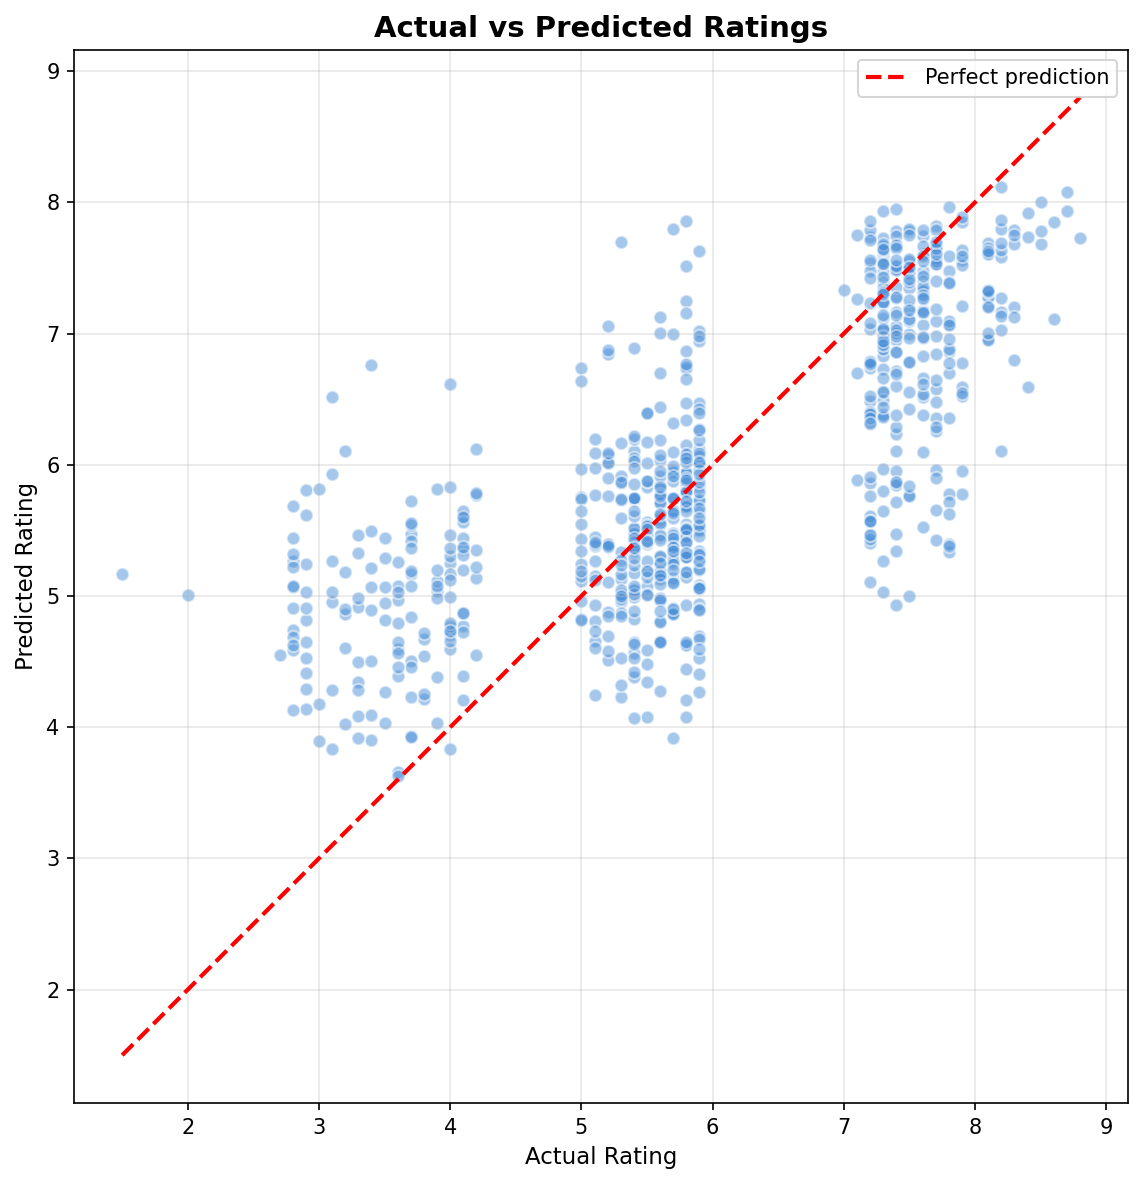
\includegraphics[width=0.78\linewidth]{../figures/05_actual_vs_predicted.png}
\caption{Actual vs.\ predicted ratings on the held-out test set
(no-weight SBERT, single-split). Predicted values concentrate
between 4 and 8 -- consistent with squared-loss regression on a
target with both heavy mass in the middle and structural empty
intervals in $[4.3, 5.0)$ and $[6.0, 7.0)$.}
\label{fig:scatter}
\end{figure}

\begin{figure}[t]
\centering
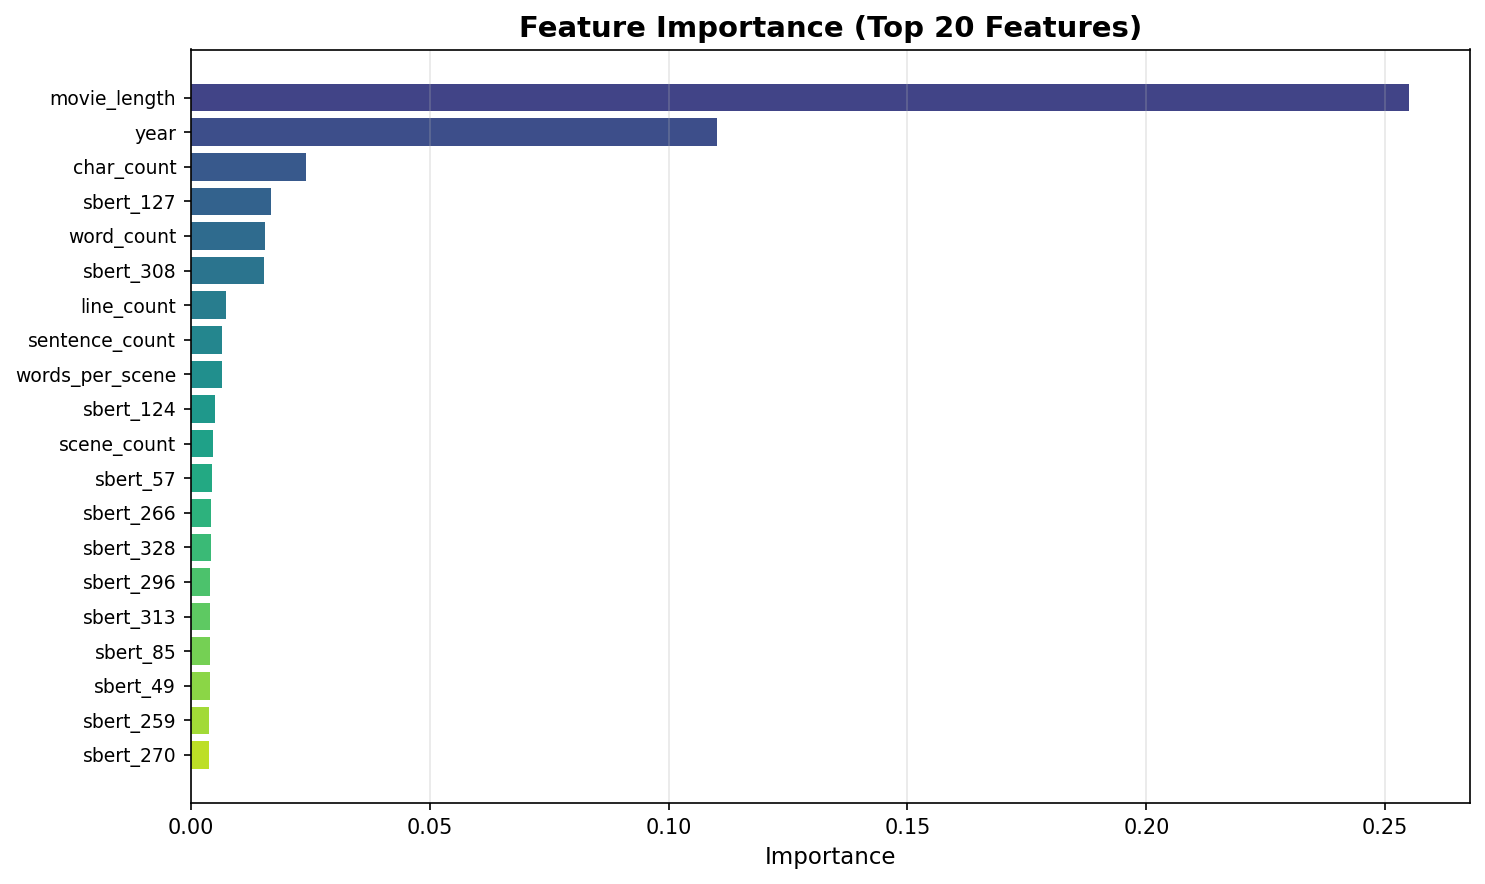
\includegraphics[width=0.85\linewidth]{../figures/04_feature_importance.png}
\caption{XGBoost feature importance (top 20). \texttt{movie\_length}
and \texttt{year} dominate; individual SBERT dimensions each
contribute less than 0.02 -- consistent with the metadata-
decomposition result that 70\% of $R^{2}$ is recoverable from
three metadata features.}
\label{fig:featimp}
\end{figure}

\begin{figure}[t]
\centering
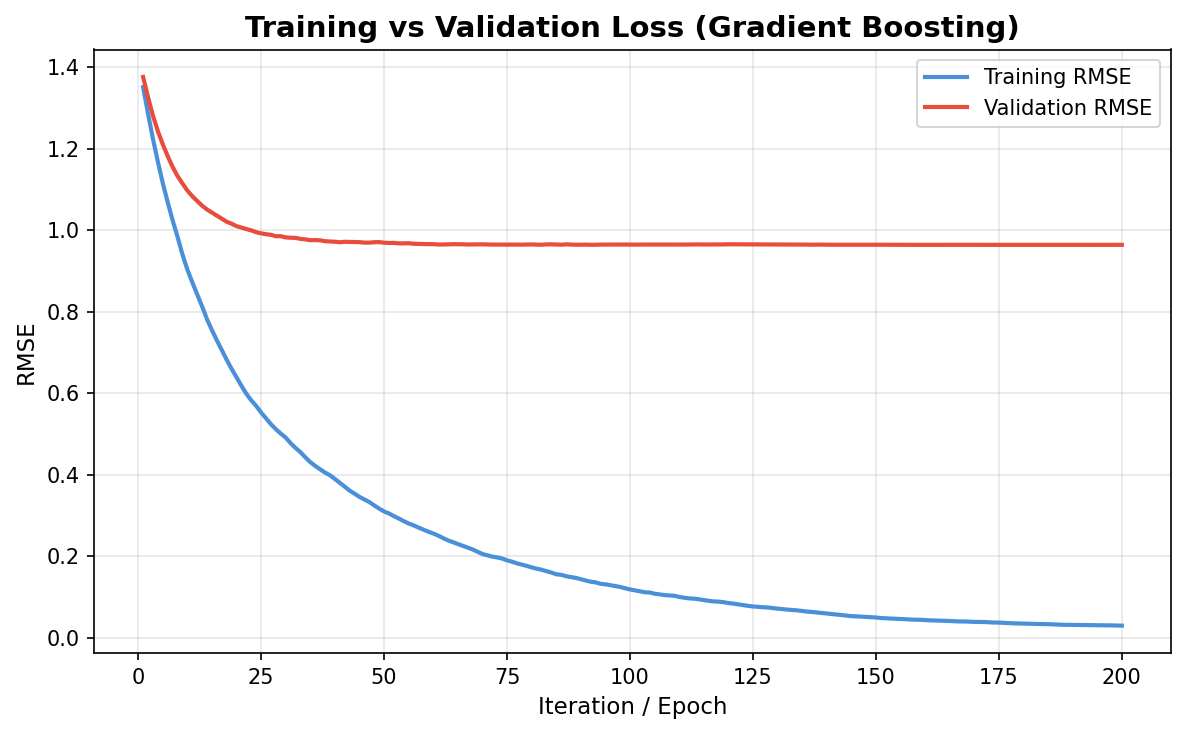
\includegraphics[width=0.78\linewidth]{../figures/02_training_validation_loss.png}
\caption{Training and validation RMSE per boosting iteration. The
early-stopping configuration in \eqref{eq:xgb-loss} prevents the
unconstrained over-fitting visible in the legacy pipeline (training
RMSE approached 0.03 while validation plateaued near 0.97).}
\label{fig:trainval}
\end{figure}

% =============================================================
%  6  DISCUSSION
% =============================================================
\section{Discussion}

The headline $5$-fold $R^{2} \approx 0.58$ is consistent with a
moderately useful predictor of audience reception from screenplay
content. It is not, however, evidence that an audience rating is
``in the script'': three metadata features alone already explain
$R^{2} \approx 0.38$ on the same corpus and splits. The
$\Delta R^{2} \approx +0.18$ attributable to script content (SBERT
+ structural features) is statistically robust but places a hard
ceiling on how much an audience rating can be claimed to
``recover from the screenplay.''

Two corollaries follow. First, papers in this area should report
metadata-only OLS as a mandatory baseline; without it, reported
$R^{2}$ values systematically over-attribute predictive power to
the text component. Second, for downstream practitioners, the
\emph{delta} over a metadata baseline, not the absolute $R^{2}$,
is the relevant figure of merit.

The negative result on inverse-frequency sample weighting is also
notable. The most up-weighted bucket (Excellent, $13.24\times$
weight) contains only 147 training samples; amplifying its
gradients makes the gradient-boosted regressor sensitive to a
high-leverage minority. Removing the reweighting also improves
per-bucket MAE on Low, suggesting the legacy weighting did not
deliver the rebalancing it was designed to produce.

% =============================================================
%  7  LIMITATIONS
% =============================================================
\section{Limitations}

\noindent\textbf{Selection bias.}
The corpus is editorially curated; rating intervals $[4.3, 5.0)$
and $[6.0, 7.0)$ are entirely empty. Generalization claims are
scoped to IMSDb-style films, not arbitrary IMDb draws.

\noindent\textbf{Metadata dominance.}
Our pipeline does not include a metadata-removed ablation
isolating the SBERT contribution from year, length, and decade
alone. The closest available comparison
(\texttt{ols\_structural}, which still contains those three
features) achieves $R^{2} = 0.44$; a controlled metadata-removed
ablation is the most important missing experiment.

\noindent\textbf{Single encoder, single pooling.}
We report \texttt{all-MiniLM-L6-v2} with mean-pooling. A larger
encoder (\texttt{all-mpnet-base-v2}) and alternative pooling
operators (max, $\ell_{2}$-weighted) are queued; our refactored
embedding cache supports them without re-encoding.

\noindent\textbf{No properly-controlled long-document transformer
baseline.}
A fair Longformer comparison (matched feature budget, full
$4{,}096$-token context) requires GPU resources beyond the
present scope.

\noindent\textbf{Rating subjectivity.}
IMDb ratings reflect production values, marketing, cast and
director reputation, and voter selection beyond the screenplay.
The unexplained variance ($1 - R^{2} \approx 0.42$) plausibly
contains a sizeable irreducible component.

% =============================================================
%  8  CONCLUSION
% =============================================================
\section{Conclusion}

We presented a screenplay-to-IMDb-rating predictor combining
frozen SBERT embeddings, hand-crafted structural features,
gradient boosting, and a Ridge meta-regressor stacked over four
base models, and evaluated it under both single-split and $5$-fold
CV protocols with bootstrap CIs and paired Wilcoxon tests. The
stacked system attains $R^{2} = 0.577 \pm 0.010$ ($5$-fold CV),
significantly improving on the strongest single base model
($p \approx 4 \times 10^{-6}$). We documented (i)~that
approximately 70\% of explained variance is recoverable from
three metadata features, (ii)~a negative result on
inverse-frequency sample weighting, (iii)~complementary signal
across base models confirmed by stacked variance, and (iv)~corpus
selection artifacts that warrant disclosure. The pipeline is
reproducible from a single command, runs in minutes on CPU, and
produces a deployable 2\,MB model.

Future work: a metadata-removed ablation; a properly-controlled
long-document transformer baseline; alternative pooling operators
using the released chunk-cache; evaluation on out-of-corpus
screenplays.

% =============================================================
%  Acknowledgments + AI disclosure + COI
%  (Springer required for proceedings)
% =============================================================

\subsubsection*{Acknowledgments.}
[Fill: funding sources, lab support, compute resources.]

\subsubsection*{Use of AI assistance.}
[Fill per Springer policy. Example: Portions of this manuscript
were drafted with the assistance of generative AI tools for
prose scaffolding and language editing. All technical content,
experiments, statistical analyses, and conclusions were designed,
executed, and verified by the authors. The authors take full
responsibility for the integrity of the work.]

\subsubsection*{Disclosure of Interests.}
The authors have no competing interests to declare that are
relevant to the content of this article.

% =============================================================
%  REFERENCES  (LNCS style)
% =============================================================
\begin{thebibliography}{99}

\bibitem{ref1}
Beltagy, I.\ et al.: Longformer: The long-document transformer.
\emph{arXiv preprint} arXiv:2004.05150 (2020)

\bibitem{ref2}
Reimers, N., Gurevych, I.: Sentence-BERT: Sentence embeddings
using Siamese BERT-networks. In: \emph{Proc.\ EMNLP}. ACL (2019)

\bibitem{ref3}
Eliashberg, J.\ et al.: Assessing box office performance using
movie scripts: A kernel-based approach. \emph{IEEE Trans.\ Knowl.\
Data Eng.} (2014)

\bibitem{ref4}
Hunter, S.D.\ et al.: Predicting box office from the screenplay:
A text analytical approach. West East Institute (2016)

\bibitem{ref5}
Reagan, A.J.\ et al.: The emotional arcs of stories are dominated
by six basic shapes. \emph{EPJ Data Science} 5(31) (2016)

\bibitem{ref6}
Ramakrishna, A.\ et al.: Linguistic analysis of differences in
portrayal of movie characters. In: \emph{Proc.\ ACL}. ACL (2017)

\bibitem{ref7}
Cini, K.: Forecasting film audience ratings: A natural language
processing approach to script and production data.
\emph{Entertainment Computing} (2025)

\bibitem{ref8}
Gross, J.A., Roberson, T.: Film success prediction using NLP
techniques. Stanford CS230 Project (2021)

\bibitem{ref9}
Kim, Y.J.\ et al.: Prediction of movie success from plot summaries
using deep learning. In: \emph{ACL Workshop} (2019)

\bibitem{ref10}
Shafaei, M.\ et al.: Age suitability rating: Predicting MPAA
rating based on movie dialogues. In: \emph{LREC} (2020)

\bibitem{ref11}
Zhang, Y.\ et al.: From none to severe: Predicting severity in
movie scripts. In: \emph{Findings of EMNLP} (2021)

\bibitem{ref12}
Chu, E., Roy, D., Glass, J.: Audio-visual sentiment analysis for
learning emotional arcs in movies. In: \emph{ICCV} (2017)

\bibitem{ref13}
Hipson, W.E.\ et al.: Emotion dynamics in movie dialogues.
\emph{PLoS ONE} (2021)

\bibitem{ref14}
Elkins, K.: Beyond plot: How sentiment analysis reshapes narrative
structure. \emph{Cultural Analytics} (2025)

\bibitem{ref15}
Sharda, R., Delen, D.: Predicting box-office success of motion
pictures with neural networks. \emph{Expert Systems with
Applications} (2006)

\bibitem{ref16}
Madongo, C.T.\ et al.: Movie box-office revenue prediction model
by mining deep features from trailers using recurrent neural
networks. \emph{J.\ Advances in Information Technology} (2024)

\bibitem{ref17}
Bhadrashetty, A., Patil, S.: Movie success and rating prediction
using data mining. \emph{J.\ Sci.\ Res.\ Tech.} (2024)

\bibitem{ref18}
Naeem, M.Z.\ et al.: Classification of movie reviews using
sentiment analysis (2022)

\bibitem{ref19}
Chalkidis, I.\ et al.: An exploration of hierarchical attention
transformers. \emph{arXiv preprint} (2022)

\bibitem{ref20}
Joshi, D.\ et al.: Pre-release critique text features for revenue
prediction

\bibitem{ref21}
Asur, S., Huberman, B.A.: Predicting the future with social media.
In: \emph{WWW} (2010)

\bibitem{ref22}
Oghina, A.\ et al.: Predicting IMDb movie ratings using Twitter
(2012)

\bibitem{ref23}
Mishne, G., Glance, N.: Predicting movie sales from blogger
sentiment. In: \emph{AAAI Spring Symposium} (2006)

\bibitem{ref24}
Mest{\'y}an, M.\ et al.: Early prediction of movie box office
success based on Wikipedia activity big data. \emph{PLoS ONE}
(2013)

\bibitem{ref25}
Vogel, H.L.: \emph{Entertainment Industry Economics}, 10th edn.
Cambridge University Press (2020)

\bibitem{ref26}
Bristi, W.R.\ et al.: Predicting IMDb rating of movies by machine
learning techniques. In: \emph{IEEE} (2019)

\bibitem{ref27}
Gomes, A.L.\ et al.: Predicting IMDb rating of TV series with
deep learning: The case of Arrow. \emph{arXiv preprint} (2022)

\bibitem{ref28}
Ramos, J.\ et al.: Movie rating prediction using sentiment
features. In: \emph{SALLD} (2022)

\bibitem{ref29}
Udandarao, V.\ et al.: Movie revenue prediction using machine
learning models. \emph{arXiv preprint} (2024)

\bibitem{ref30}
Xie, W.\ et al.: Predicting movie success with multi-task
learning: GPT-based sentiment and SIR propagation.
\emph{arXiv preprint} (2025)

\bibitem{ref31}
Balestri, R.\ et al.: An automatic deep learning approach for
trailer generation through large language models.
\emph{arXiv preprint} (2026)

\bibitem{ref32}
Sharma, A.S.\ et al.: Presenting a larger up-to-date movie
dataset. \emph{arXiv preprint} (2021)

\bibitem{ref33}
Ding, Y.\ et al.: A machine learning model based on data-driven
movie derivatives market prediction. \emph{arXiv preprint} (2022)

\bibitem{ref34}
Mohamed, E.\ et al.: A first dataset for film age appropriateness
investigation. In: \emph{LREC} (2020)

\bibitem{ref35}
Kar, S.\ et al.: Folksonomication: Predicting tags for movies from
plot synopses using emotion flow encoded neural network. In:
\emph{COLING} (2018)

\bibitem{ref36}
Tixier, A.J.P.: Notes on deep learning for NLP.
\emph{arXiv preprint} (2018)

\bibitem{ref37}
Pal, A.\ et al.: Identifying movie genre compositions using
neural networks. In: \emph{IEEE} (2020)

\bibitem{ref38}
Chiu, M.C.\ et al.: Screenplay quality assessment: Can we predict
who gets nominated? NUSe (2020)

\end{thebibliography}

\end{document}
